\documentclass[pdftex,12pt,a4paper]{report}

\usepackage[portuguese,english]{babel}
\usepackage[T1]{fontenc} 
\usepackage[utf8]{inputenc}
\usepackage[pdftex]{graphicx}
\usepackage{minitoc}
\usepackage{hyperref}
\usepackage{indentfirst}
\usepackage[compact]{titlesec}
\usepackage{fancyhdr}
\usepackage{caption}
\usepackage{pgfplots}
\usepackage{pgfplotstable}
\usepackage{fixltx2e}
\usepackage{mathtools}
\pagestyle{fancy}
\fancyhead{}
\renewcommand*\thesection{\thechapter\arabic{section}}
\newcommand{\HRule}{\rule{\linewidth}{0.5mm}}
\begin{document} 

\begin{titlepage}

\begin{center}


\includegraphics[width=0.15\textwidth]{./logo}\\[0.5cm]    

\textsc{\large Universidade de Aveiro \\[1cm]\large departamento de electrónica, telecomunicações e informática}\\[1cm]

\textsc{\large{41541}\large - Sistemas Electrónicos \\[1cm]}

\HRule \\[0.5cm]
{ \huge \bfseries Relatório Trabalho Prático Nº2}\\[0.4cm]
\HRule \\[1cm]

\textsc{\small{8240 - MESTRADO INTEGRADO EM ENGENHARIA DE COMPUTADORES E TELEMÁTICA}}\\[1cm]

\begin{minipage}{0.4\textwidth}

\begin{flushleft} \large
\href{mailto:rafael.ferreira@ua.pt}{António Rafael da \\ Costa Ferreira }
 \small{\\NMec: 67405 | P3}
\end{flushleft}
\end{minipage}
\begin{minipage}{0.4\textwidth}

\begin{flushright} \large
\href{mailto:rodrigocunha@ua.pt}{Rodrigo Lopes \\ da Cunha}
\small{\\NMec: 67800 | P3}
\end{flushright}
\end{minipage}\\[1cm]

{\large Docente:  João Pedro Estima de Oliveira  }\\[0.5cm]

\vfill

{\large Maio de 2014 \\ 2013-2014}

\end{center}

\end{titlepage} %Titulo do Relatorio
\renewcommand{\headrulewidth}{0pt}

%Parte do resumo!
\vspace*{\fill}
\textbf{Introdução?? Reusmo??:}
\begingroup
normalmente a introdução é feita 
\endgroup
\vspace*{\fill}
%Parte do resumo!
\newpage

%Renomear Comandos
\renewcommand*\contentsname{Conteúdos}
\renewcommand*\figurename{Figura}

%Conteúdos, dar paragrafo
\tableofcontents
%Headers
\renewcommand{\headrulewidth}{0.15pt}
\lhead{Relatório Trabalho Prático Nº2}
\renewcommand{\thechapter}{}

\clearpage

\section{Parte I - Análise de Circuitos com Díodos}
\begin{figure}[h]
\centerline{\fbox{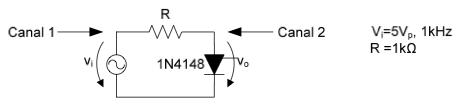
\includegraphics[width=0.5\textwidth]{./Imagens/Diodo-1parte.png}}}
\caption{Circuito com díodo para determinar a característica i-v}\label{diodo_parte1}
\end{figure}

\subsection{Característica i-v de um díodo} 
\hbox{\emph{\textbf{Pergunta 1:}}\newline\newline}

Para calcular a característica i-v de um díodo, usando os valores obtidos no osciloscópio e a fórmula $i = \frac{V\textsubscript{i}-V\textsubscript{0}}{R}$ obtemos a seguinte tabela e gráfico:\newline

\minipage{0.65\textwidth}
\begin{tikzpicture}
\begin{axis}[
    title={Gráfico da característica i-v de um díodo},
    xlabel={$v_0$ (V)},
    ylabel={i (mA)},
    xmin=-6, xmax=3,
    ymin=0, ymax=5,
    xtick={-5, -4, -2, 0, 2, 4},
    ytick={-5, -3, 0, 3, 5, 6},
    legend pos=north west,
    ymajorgrids=true,
    grid style=dashed,
]
\addplot table [y=i, x=$v_0$, color=blue, mark=square]{./diodos_data.dat};
\legend{i/v}
\end{axis}
\end{tikzpicture}
\endminipage\hfill
\minipage{0.3\textwidth}
\pgfplotstabletypeset{./diodos_data.dat}
\endminipage\hfill

\begin{figure}[h]
\centerline{\fbox{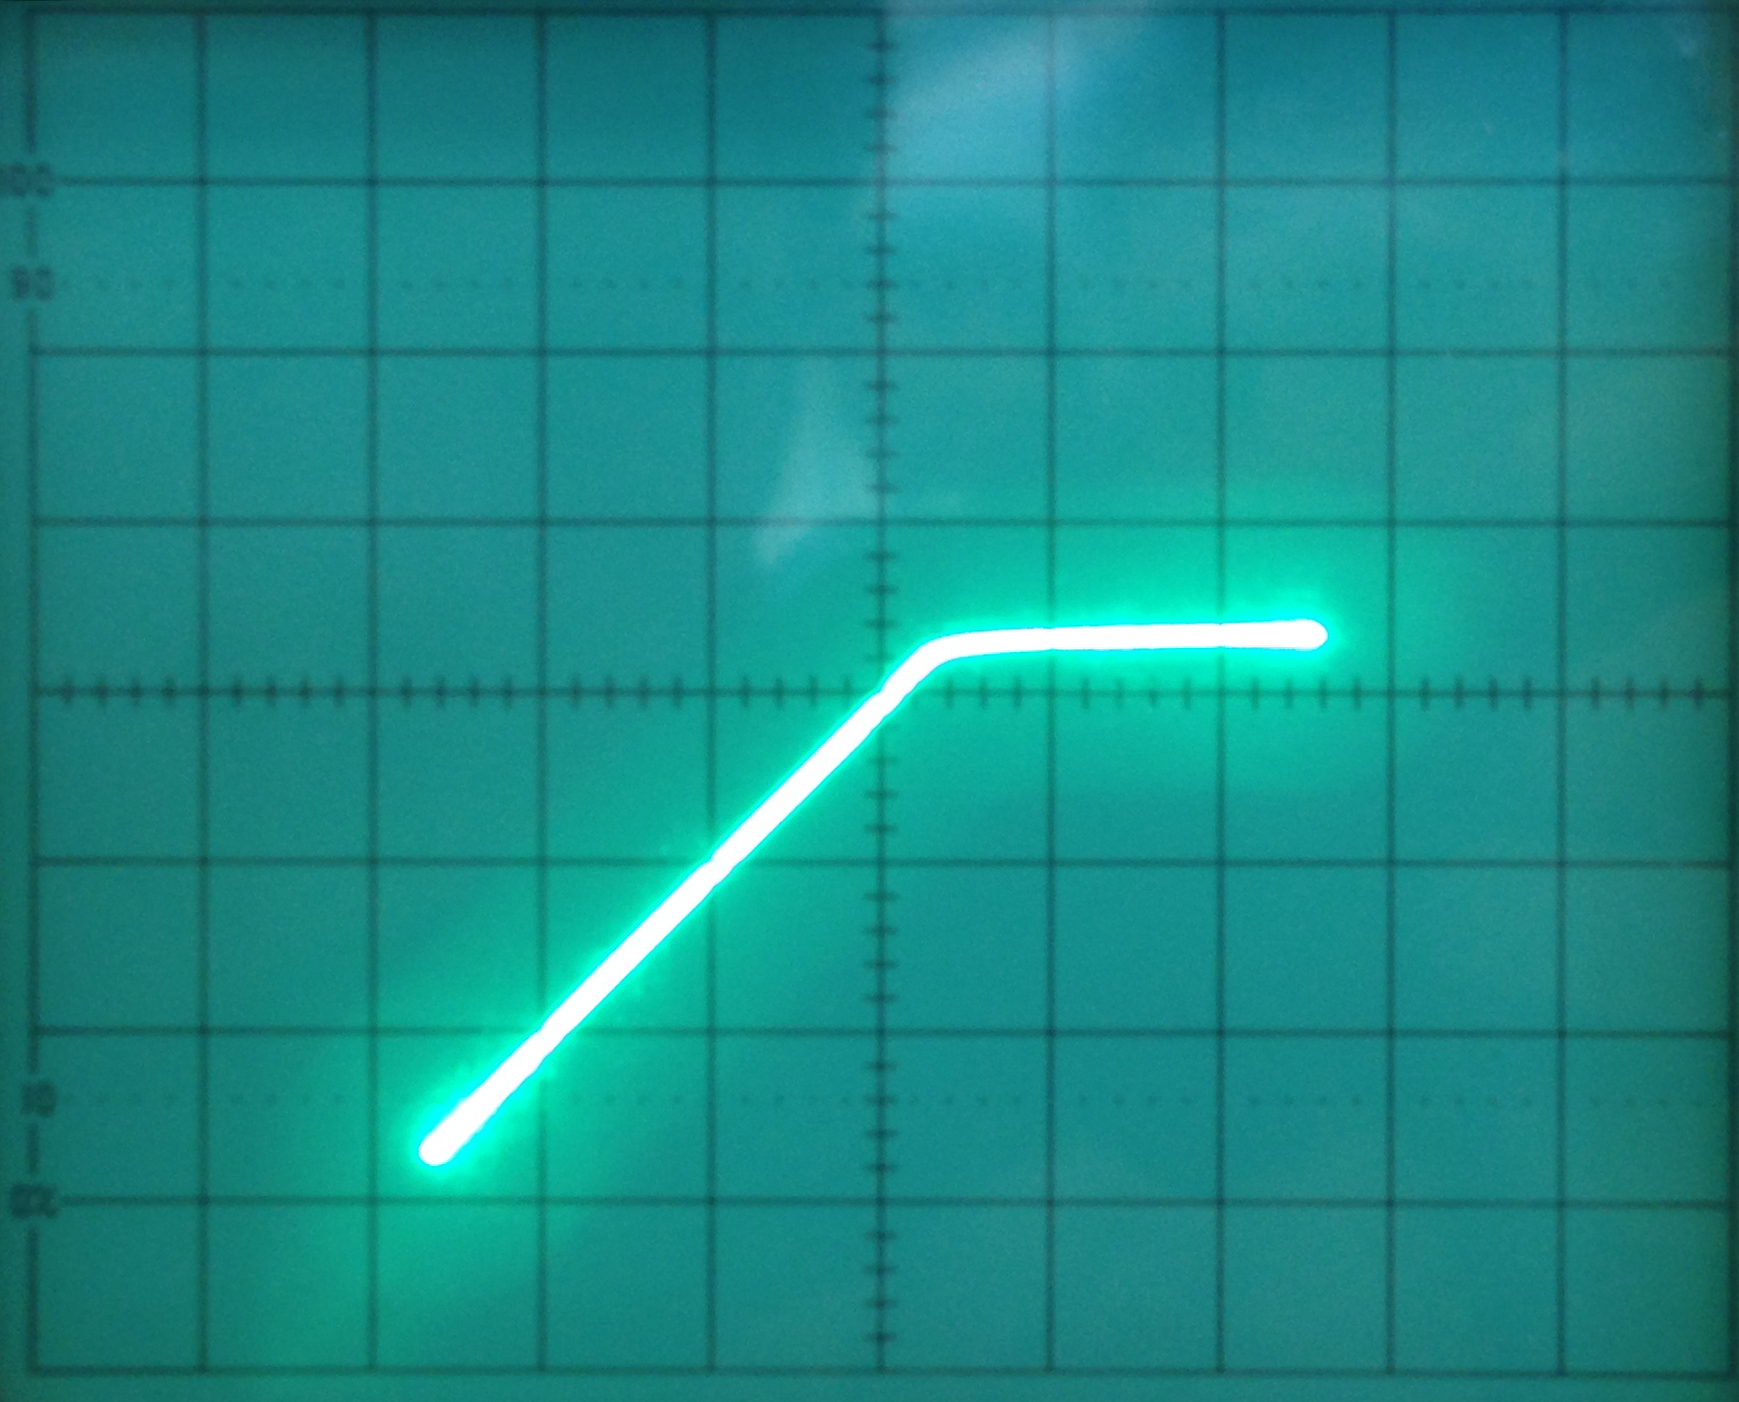
\includegraphics[width=0.35\textwidth]{./Imagens/tp2parte1c.JPG}}}
\caption{Modo \textit{xy} observado no osciloscópio (2V/div) ambos}\label{grafico_1c_osciloscopio}
\end{figure}

\clearpage
\subsection{Formas de onda de V\textsubscript{in}(t)  e V\textsubscript{out}(t) quando a amplitude de V\textsubscript{in}(t) = 0.2V e de V\textsubscript{in}(t) = 2V}
\hbox{\emph{\textbf{Pergunta 2:}}\newline}
As duas ondas sinusoidais coincidem, pois 0,2 V não é suficiente para fazer o díodo conduzir, por isso a tensão do canal 2 é igual à do canal 1:

\begin{figure}[h]
\centerline{\fbox{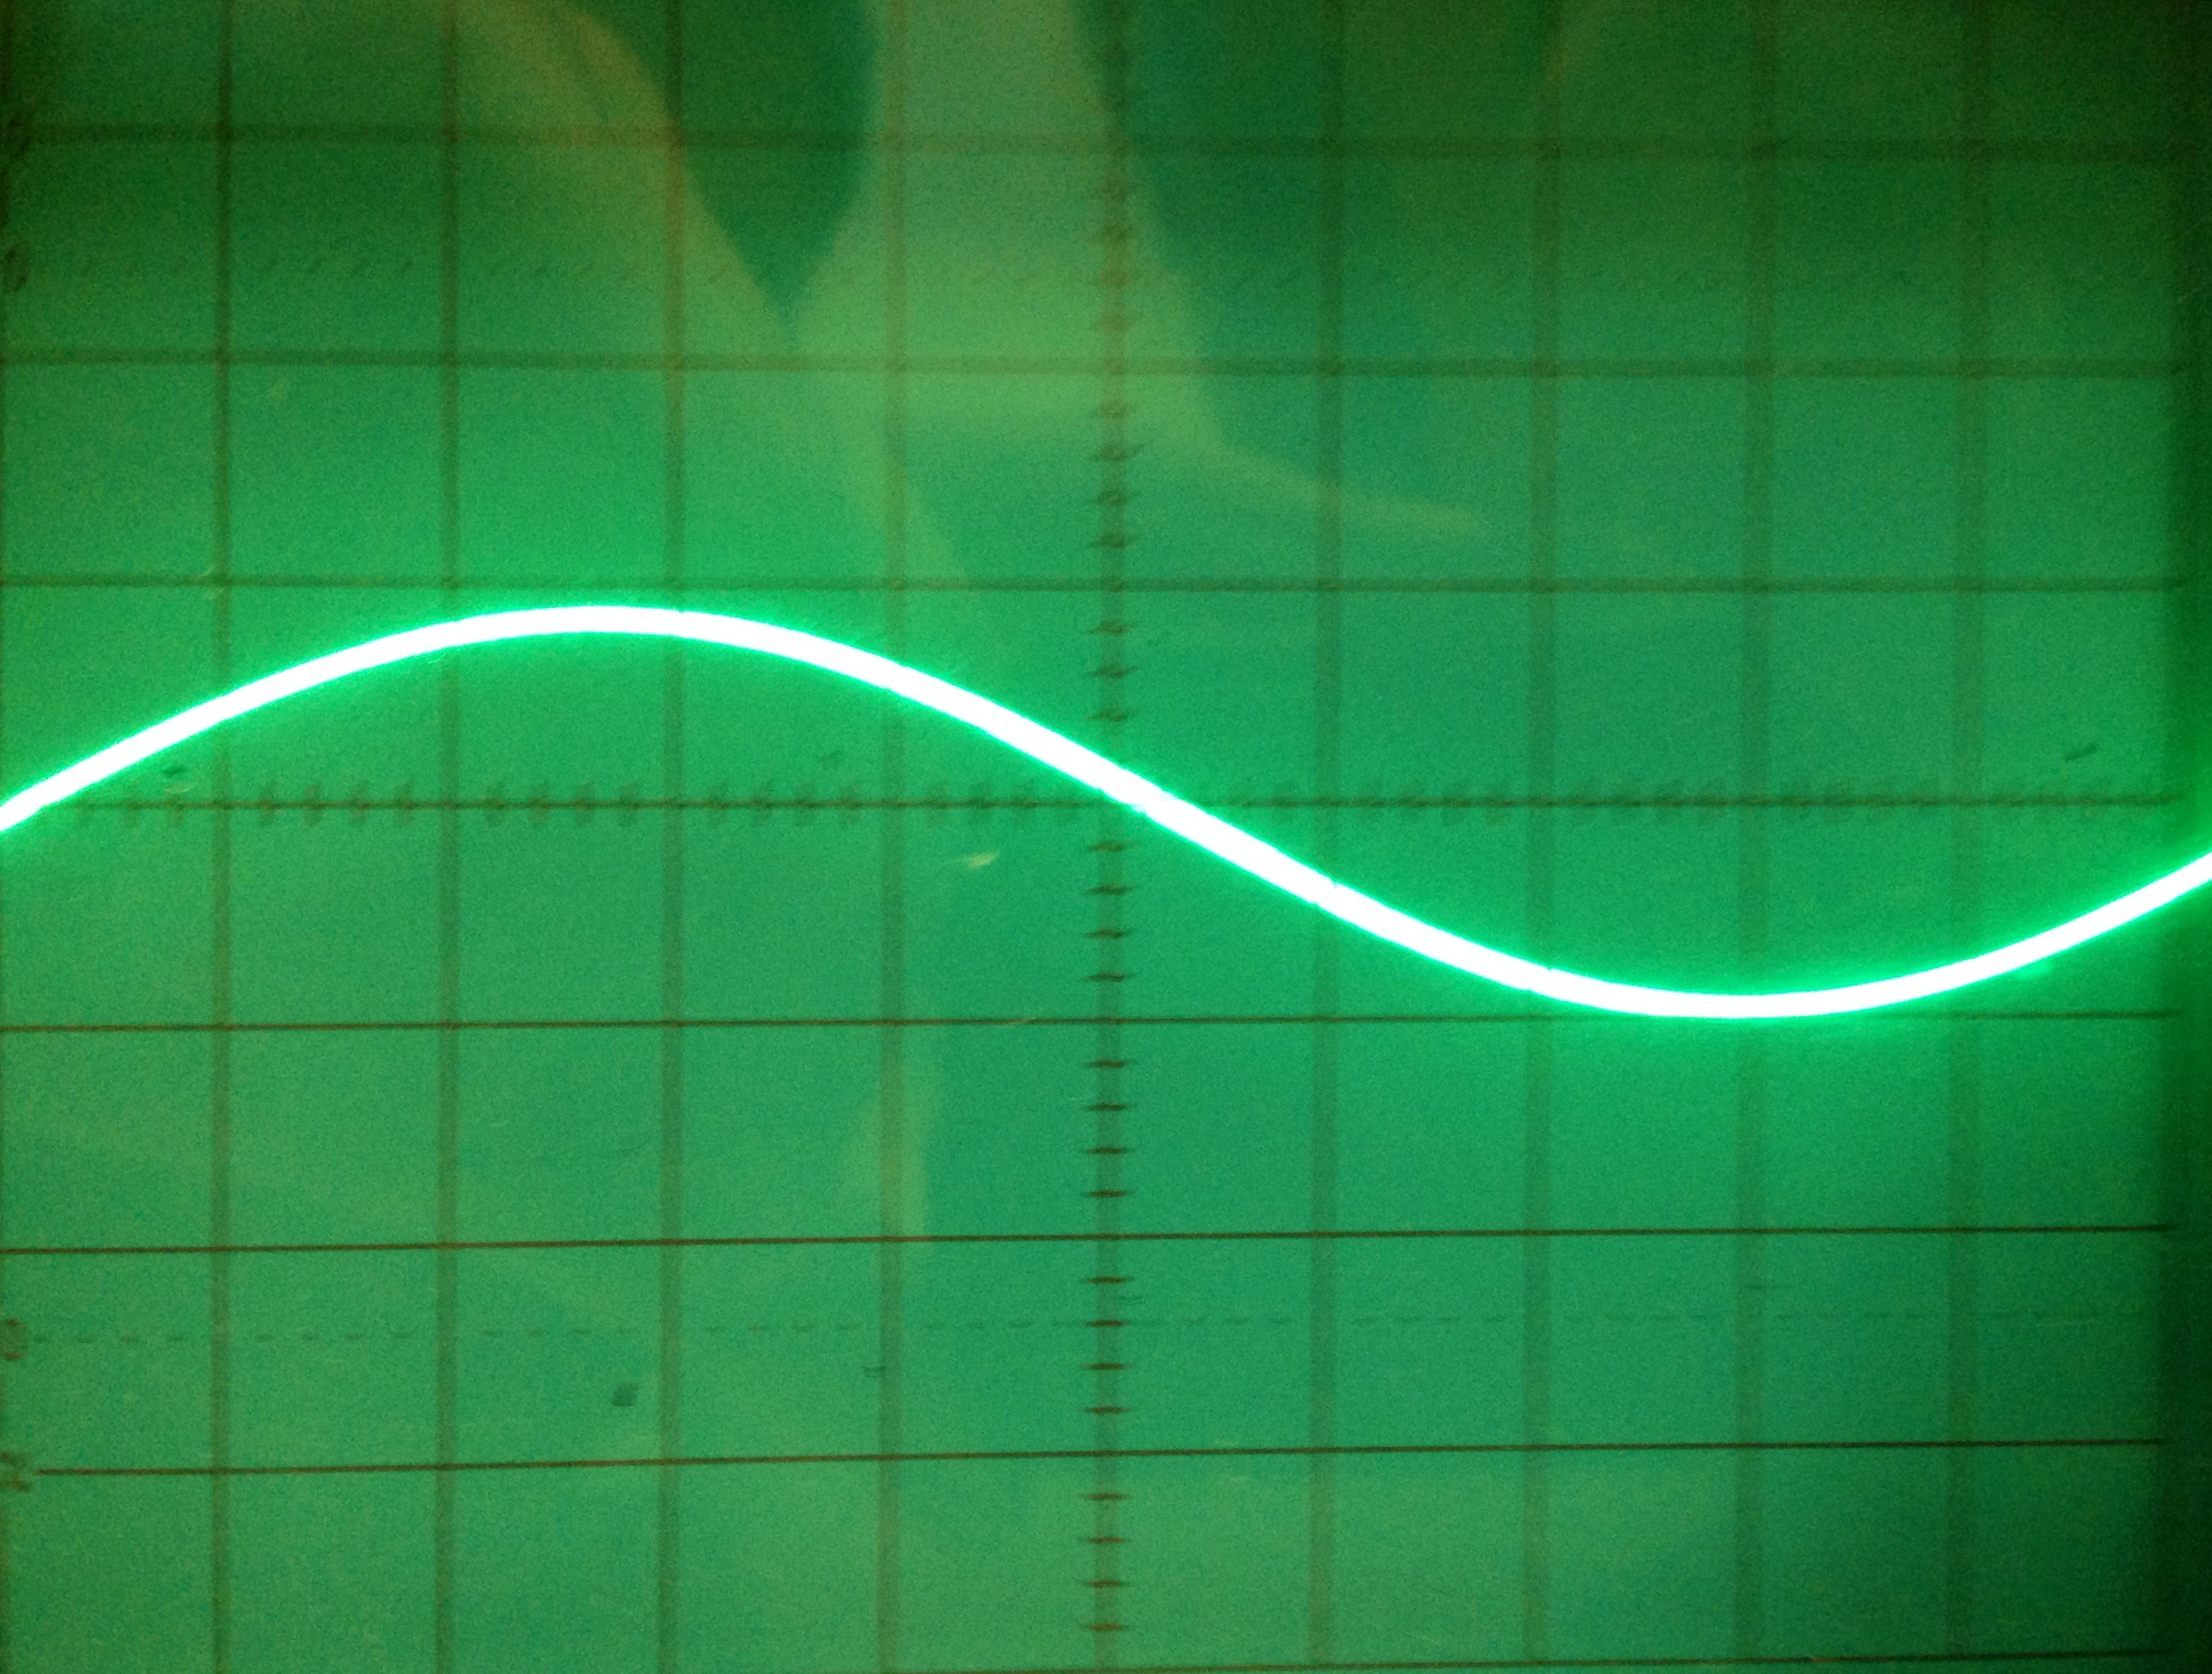
\includegraphics[width=0.6\textwidth]{./Imagens/parte1_ex2_02v_1.jpg}}}
\caption{Vertical: 0,1V/div (ambos); Horizontal: 0,1ms/div(A), 1$\mu$s/div(B)}\label{grafico_12_02_osciloscopio}
\end{figure}

O díodo limita a tensão do canal 2 para 0,7V (tal como determinado na pergunta 1), sendo a tensão no canal 1 de 2V. Podemos verificar este feito na imagem seguinte: 

\begin{figure}[h]
\centerline{\fbox{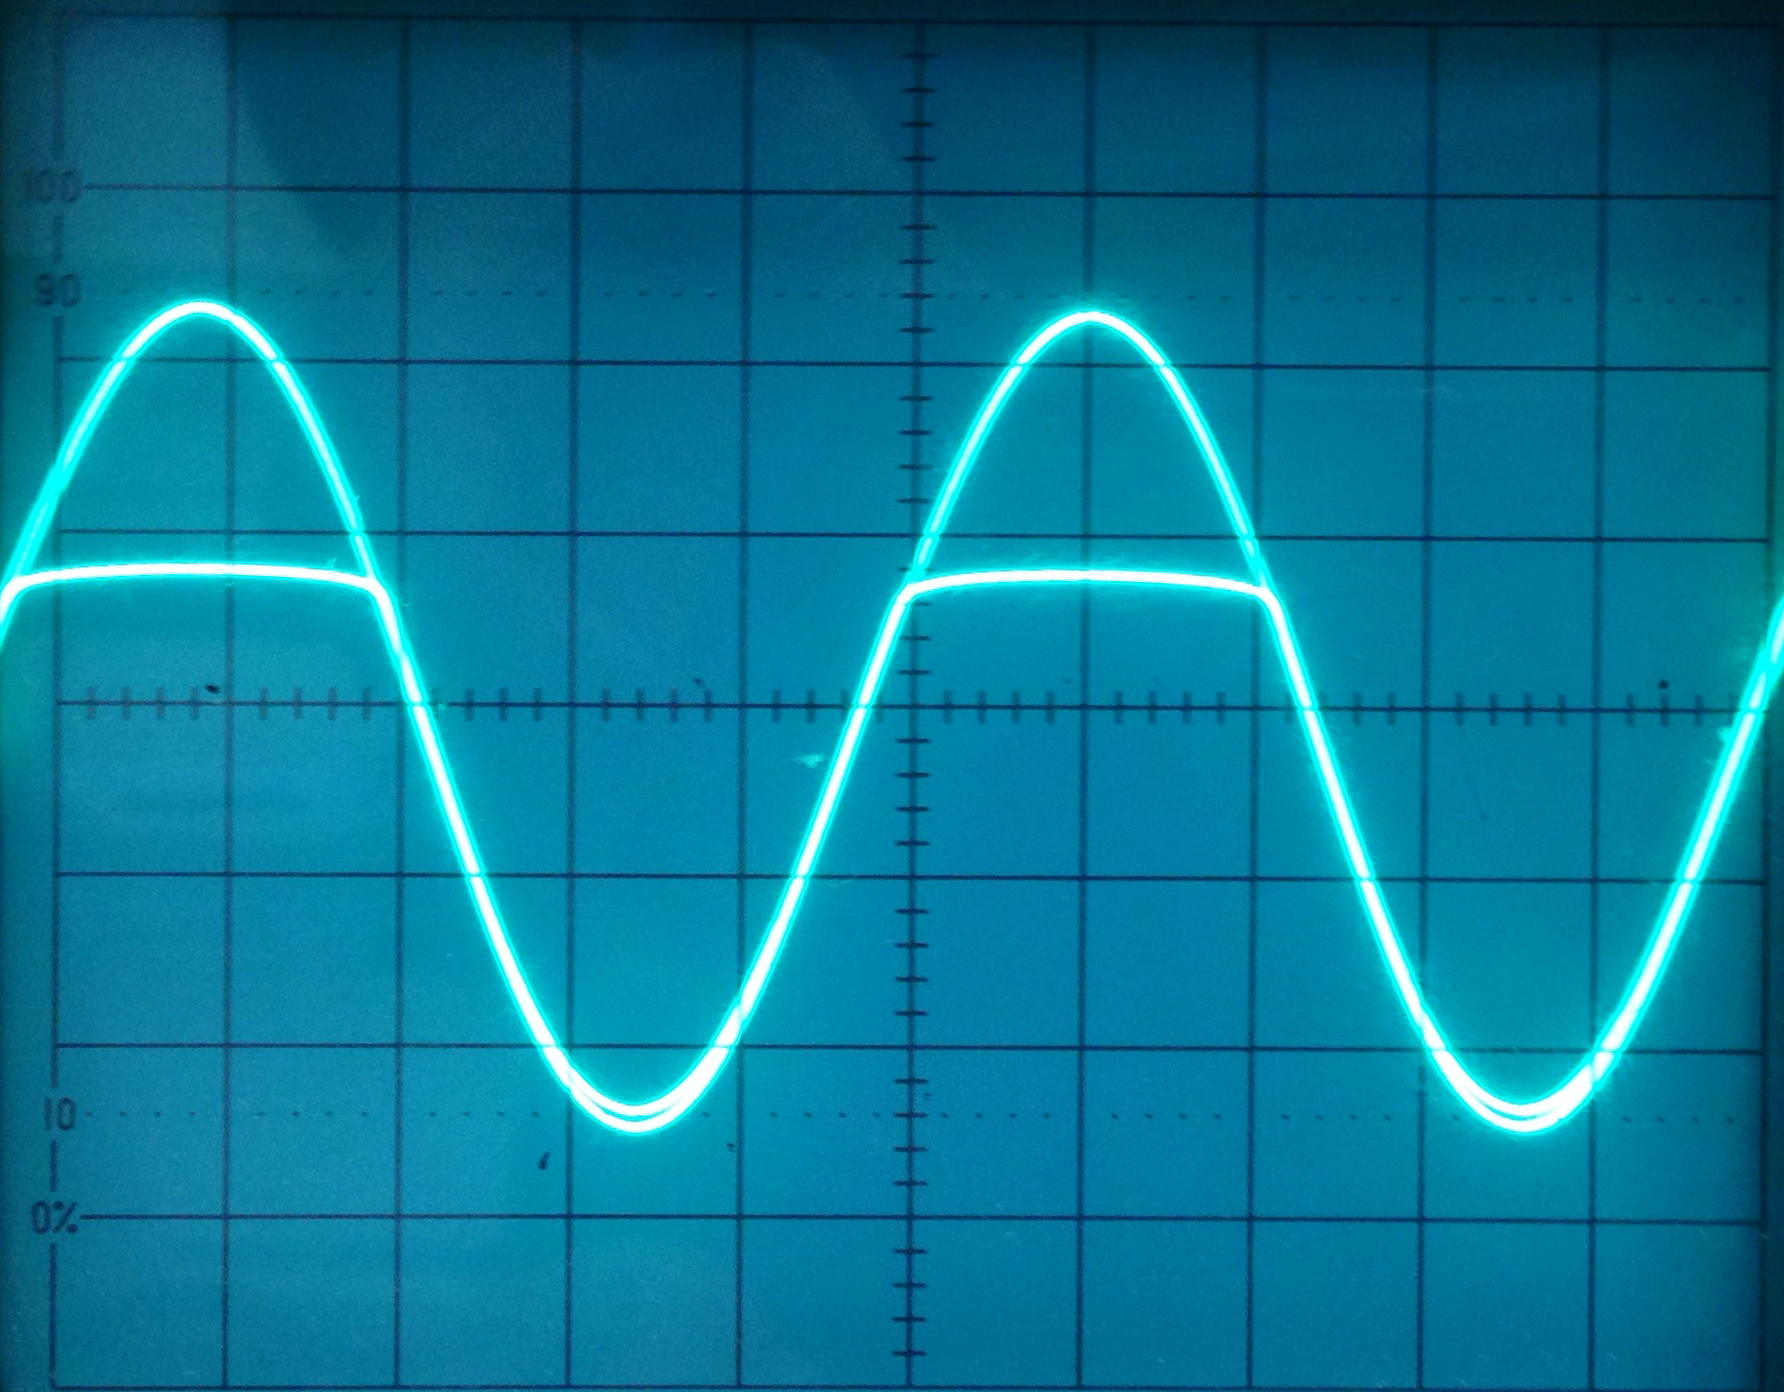
\includegraphics[width=0.6\textwidth]{./Imagens/parte1_ex2_2v_1.jpg}}}
\caption{}\label{grafico_12_02_osciloscopio}
\end{figure}

\subsection{Circuitos limitadores com díodos}
\hbox{\emph{\textbf{Pergunta 3:}\newline}}

\begin{figure}[h]
\centerline{\fbox{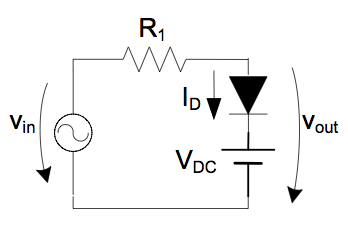
\includegraphics[width=0.35\textwidth]{./Imagens/parte1_ex3.png}}}
\caption{$V_{in}$=10V, 1kHz}\label{circuito13}
\end{figure}
Através da expressão $V = R*I_D$ obtém-se o valor de $R_1$:\newline
\centerline{$I_D = \frac{V_{in} - V_{out}}{R_1} \Leftrightarrow 10^-3 = \frac{10-1,8}{R_1} \Leftrightarrow R_1 = \frac{8,2}{10^-3} \simeq 8,2k\Omega$}\\
\vspace{0.1cm}

Para obter o valor de $V_{DC}$, basta utilizar a expressão $V_{out} = V_D + V_{DC}$:
\centerline{$ 1,8 = 0,6 + V_{DC} \Leftrightarrow V_{DC} = 1,2V$}

Como podemos verificar na imagem abaixo, o circuito ficou limitado a 1,8 V como era pretendido:

\begin{figure}[h]
\centerline{\fbox{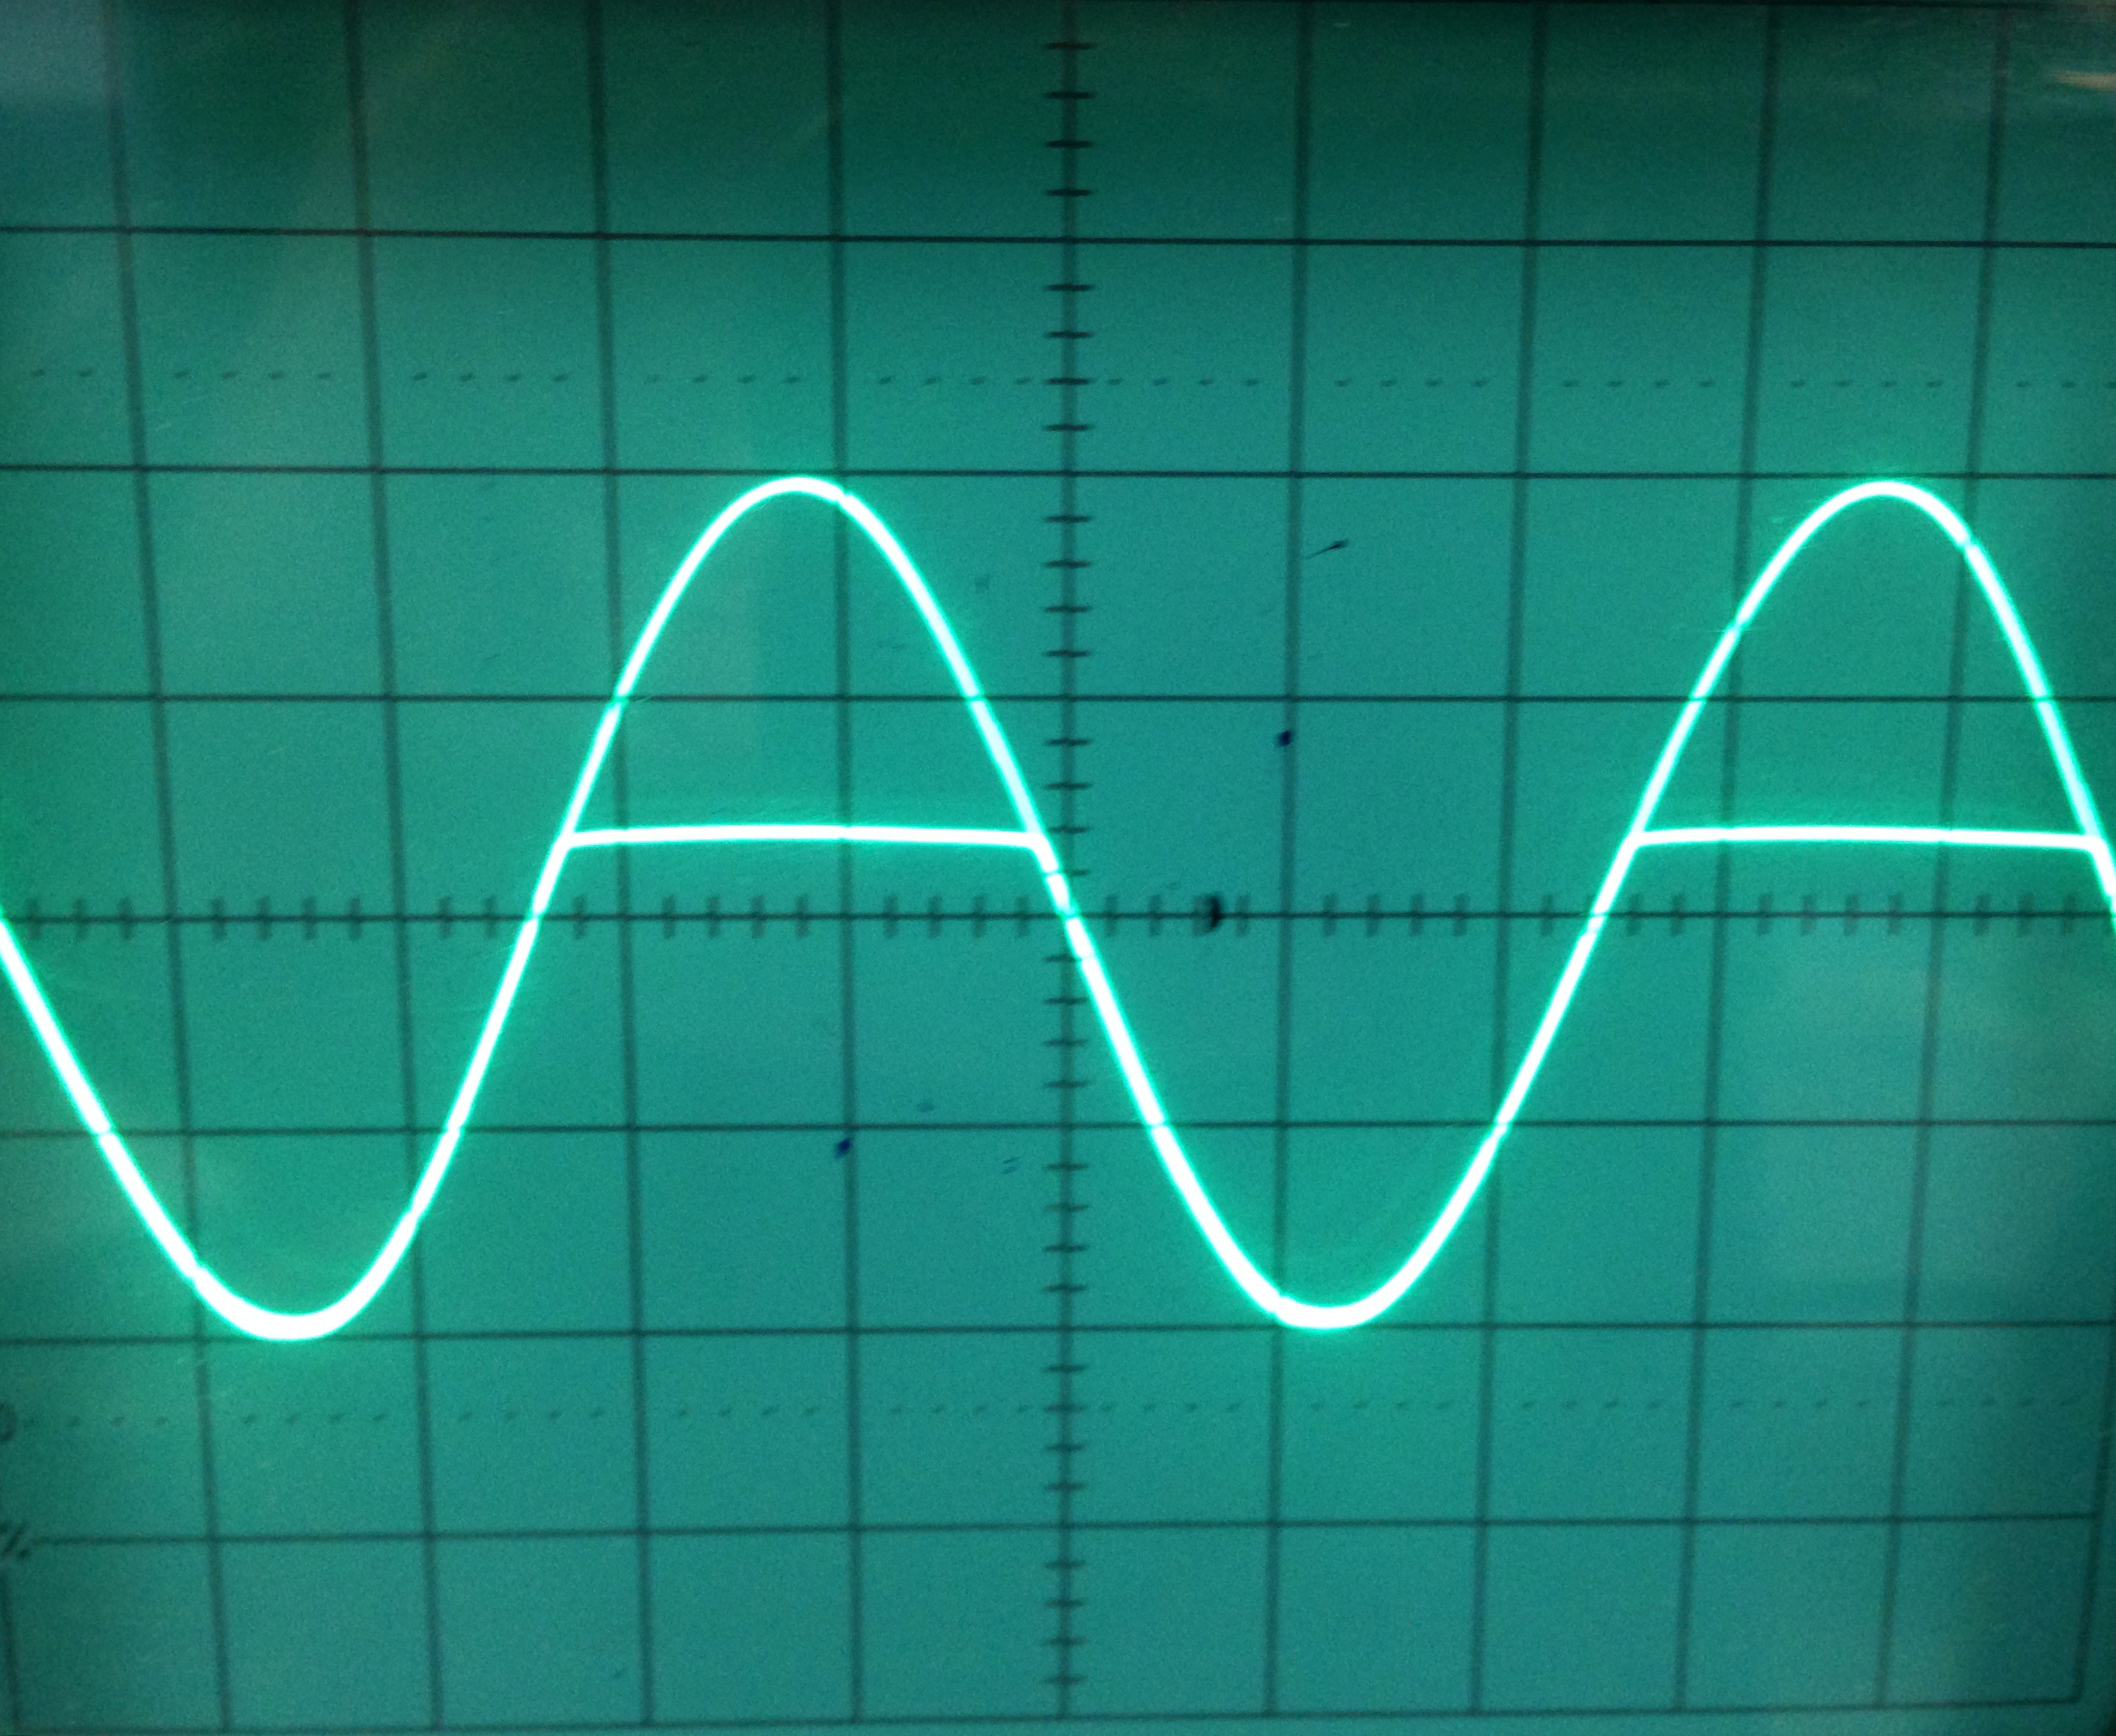
\includegraphics[width=0.55\textwidth]{./Imagens/parte1_ex3.jpg}}}
\caption{ESTA IMAGEM ESTÁ MAL TEMOS DE LA VOLTAR }\label{grafico_1c_osciloscopio}
\end{figure}

\newpage

\section{Parte II - Análise	de	Portas	Lógicas	e	Circuitos	Lógicos}

\begin{figure}[!htb]
\minipage{0.2\textwidth}
  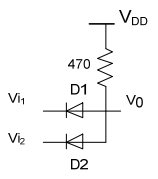
\includegraphics[width=\linewidth]{Imagens/Diodos.png}
  \caption{\\Díodo}\label{fig:fig_diodo}
\endminipage\hfill
\minipage{0.2\textwidth}
  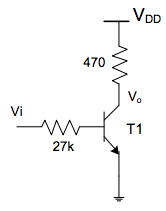
\includegraphics[width=\linewidth]{Imagens/BJT.png}
  \caption{\\BJT}\label{fig:fig_bjt}
\endminipage\hfill
\minipage{0.2\textwidth}
  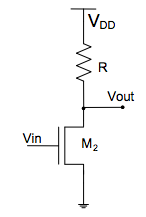
\includegraphics[width=\linewidth]{Imagens/NMOS.png}
  \caption{\\NMOS}\label{fig:fig_nmos}
\endminipage
\minipage{0.2\textwidth}
  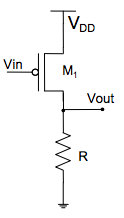
\includegraphics[width=\linewidth]{Imagens/PMOS.png}
  \caption{\\PMOS}\label{fig:fig_pmos}
\endminipage\hfill
\minipage{0.2\textwidth}
  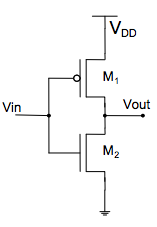
\includegraphics[width=\linewidth]{Imagens/CMOS.png}
  \caption{\\CMOS}\label{fig:fig_cmos}
\endminipage\hfill
\end{figure}

\section{Parte III - Aplicações	de	Circuitos	Lógicos	CMOS}


\end{document}